\documentclass{standalone}
\usepackage{tikz}
\usetikzlibrary{patterns, positioning}
\usepackage[sfdefault]{ClearSans} %% option 'sfdefault' activates Clear Sans as the default text font
\usepackage[T1]{fontenc}

\begin{document}
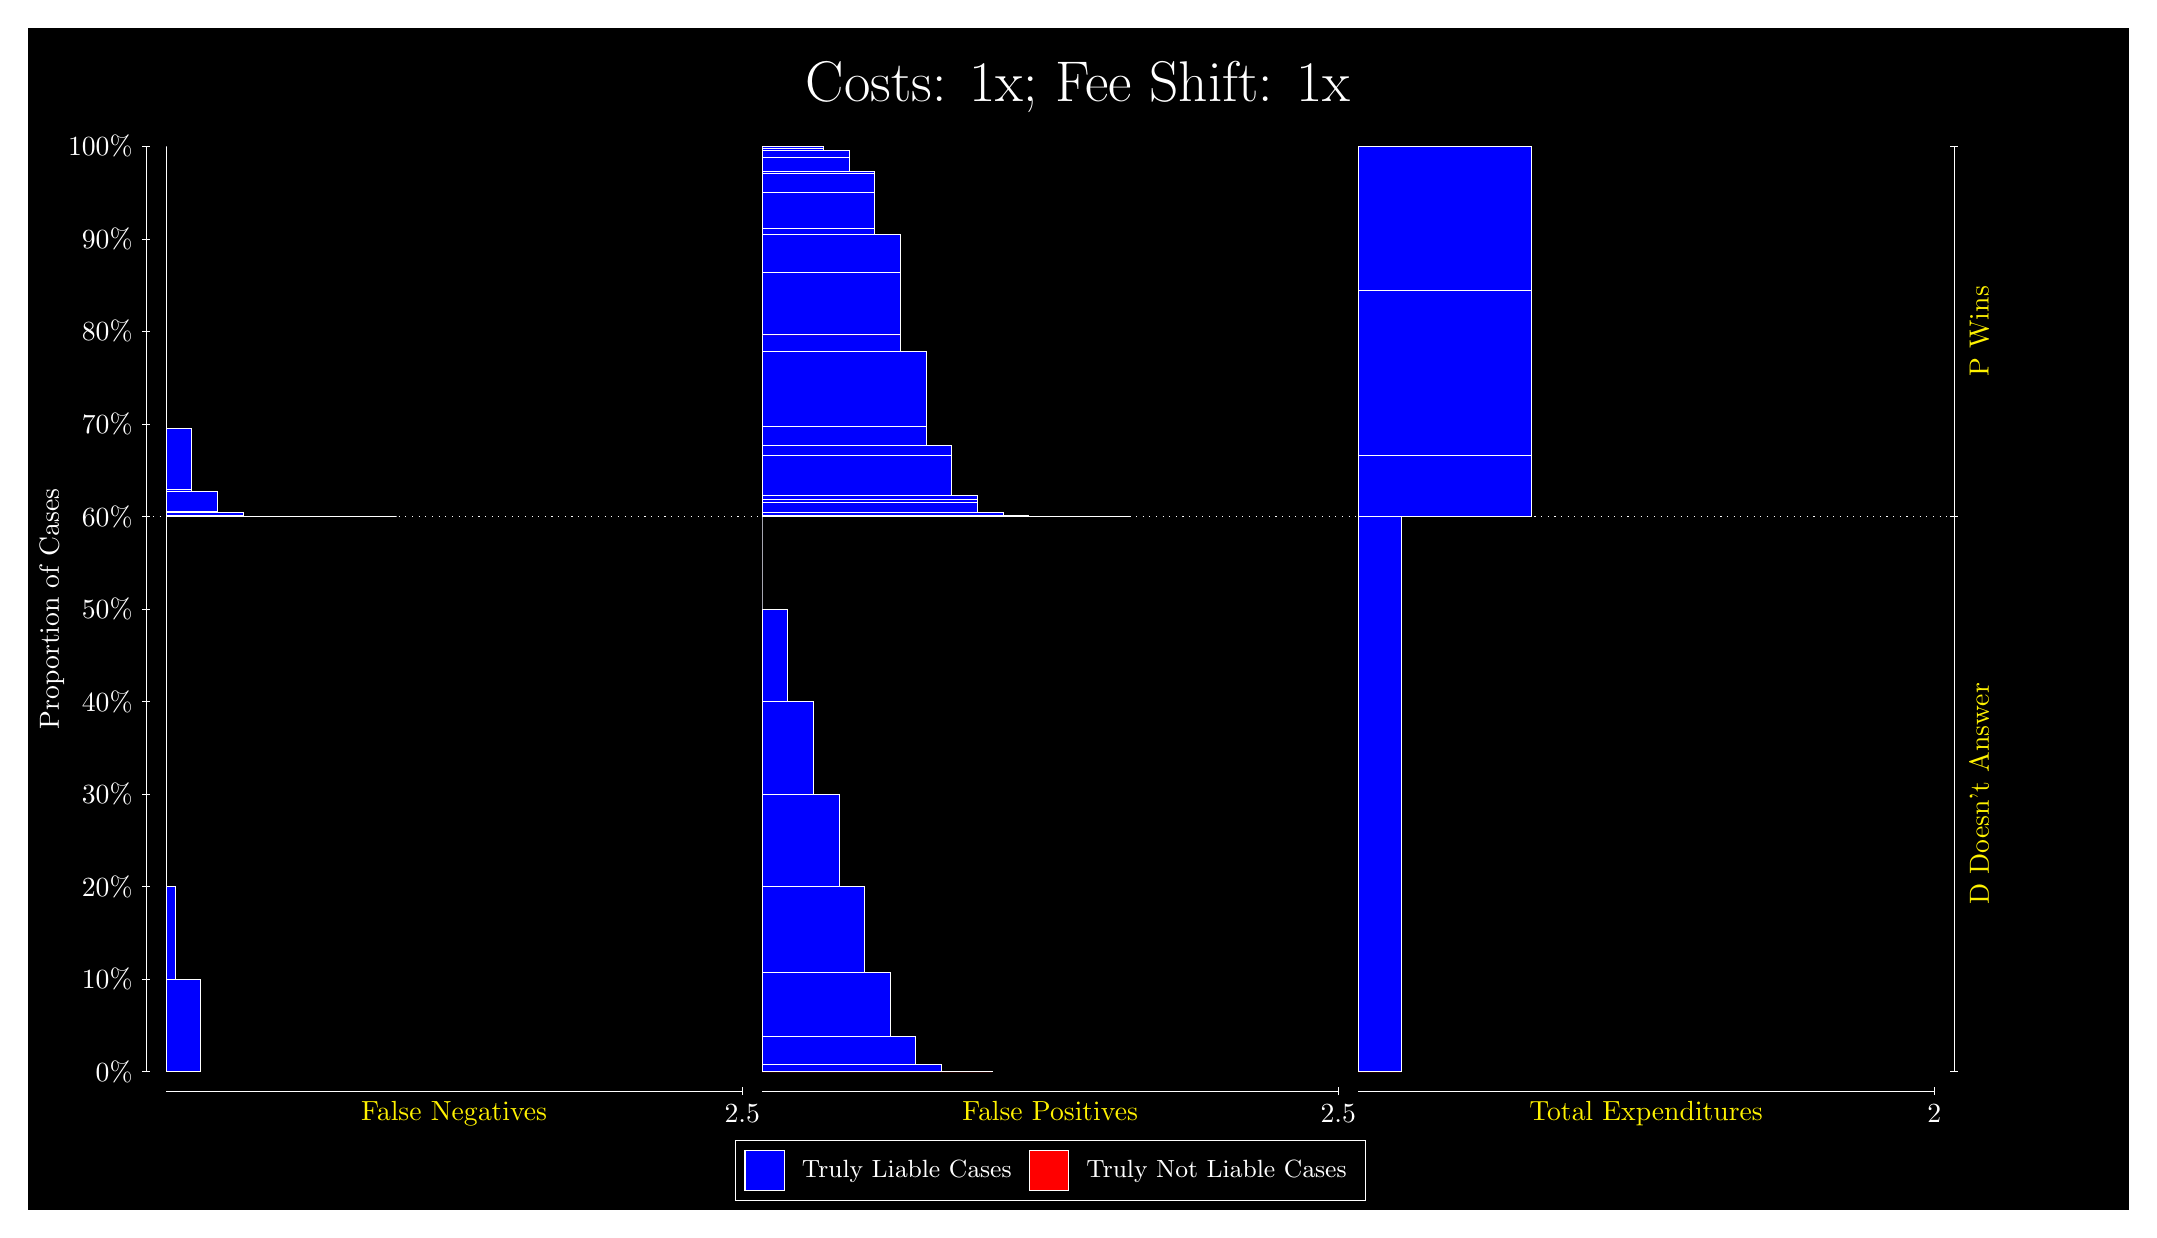
\begin{tikzpicture}
\draw[fill=black] (0,0) rectangle (26.667,15);
\draw[text=white] (0,13.5) rectangle (26.667,15) node[midway] {\huge Costs: 1x; Fee Shift: 1x};
\draw[white, very thin] (1.5,1.75) -- (1.5,13.5);
\node[rotate=90, text=white, anchor=center] at (0.3, 7.625) {Proportion of Cases};
\draw[white, very thin] (1.45,1.75) -- (1.55,1.75);
\node[text=white, anchor=east] at (1.45, 1.75) {0\%};
\draw[white, very thin] (1.45,2.925) -- (1.55,2.925);
\node[text=white, anchor=east] at (1.45, 2.925) {10\%};
\draw[white, very thin] (1.45,4.1) -- (1.55,4.1);
\node[text=white, anchor=east] at (1.45, 4.1) {20\%};
\draw[white, very thin] (1.45,5.275) -- (1.55,5.275);
\node[text=white, anchor=east] at (1.45, 5.275) {30\%};
\draw[white, very thin] (1.45,6.45) -- (1.55,6.45);
\node[text=white, anchor=east] at (1.45, 6.45) {40\%};
\draw[white, very thin] (1.45,7.625) -- (1.55,7.625);
\node[text=white, anchor=east] at (1.45, 7.625) {50\%};
\draw[white, very thin] (1.45,8.8) -- (1.55,8.8);
\node[text=white, anchor=east] at (1.45, 8.8) {60\%};
\draw[white, very thin] (1.45,9.975) -- (1.55,9.975);
\node[text=white, anchor=east] at (1.45, 9.975) {70\%};
\draw[white, very thin] (1.45,11.15) -- (1.55,11.15);
\node[text=white, anchor=east] at (1.45, 11.15) {80\%};
\draw[white, very thin] (1.45,12.325) -- (1.55,12.325);
\node[text=white, anchor=east] at (1.45, 12.325) {90\%};
\draw[white, very thin] (1.45,13.5) -- (1.55,13.5);
\node[text=white, anchor=east] at (1.45, 13.5) {100\%};

\draw[white, very thin] (24.457,1.75) -- (24.457,13.5);
\draw[white, very thin] (24.407,1.75) -- (24.507,1.75);
\node[anchor=west] at (24.407, 1.75) {};
\draw[white, very thin] (24.407,8.8012) -- (24.507,8.8012);
\node[anchor=west] at (24.407, 8.8012) {};
\draw[white, very thin] (24.407,13.5) -- (24.507,13.5);
\node[anchor=west] at (24.407, 13.5) {};

\draw[white, very thin, fill=blue] (1.75,1.75) rectangle (2.1891,2.925);
\draw[white, very thin, fill=blue] (1.75,2.925) rectangle (1.8638,4.1);
\draw[white, very thin, fill=red] (1.75,4.1) rectangle (1.75,4.1);
\draw[white, very thin, fill=blue] (1.75,4.1) rectangle (1.75,8.8012);
\draw[white, very thin, fill=blue] (1.75,8.8012) rectangle (4.6775,8.8012);
\draw[white, very thin, fill=blue] (1.75,8.8012) rectangle (4.3523,8.8012);
\draw[white, very thin, fill=blue] (1.75,8.8012) rectangle (4.027,8.8012);
\draw[white, very thin, fill=blue] (1.75,8.8012) rectangle (4.027,8.8012);
\draw[white, very thin, fill=blue] (1.75,8.8012) rectangle (3.7017,8.8012);
\draw[white, very thin, fill=blue] (1.75,8.8012) rectangle (3.7017,8.8012);
\draw[white, very thin, fill=blue] (1.75,8.8012) rectangle (3.3764,8.8014);
\draw[white, very thin, fill=blue] (1.75,8.8014) rectangle (3.0511,8.802);
\draw[white, very thin, fill=blue] (1.75,8.802) rectangle (3.0511,8.8052);
\draw[white, very thin, fill=blue] (1.75,8.8052) rectangle (2.7258,8.8082);
\draw[white, very thin, fill=blue] (1.75,8.8082) rectangle (2.7258,8.8534);
\draw[white, very thin, fill=blue] (1.75,8.8534) rectangle (2.7258,8.8534);
\draw[white, very thin, fill=blue] (1.75,8.8534) rectangle (2.4006,8.8621);
\draw[white, very thin, fill=blue] (1.75,8.8621) rectangle (2.4006,9.1218);
\draw[white, very thin, fill=blue] (1.75,9.1218) rectangle (2.0753,9.1384);
\draw[white, very thin, fill=blue] (1.75,9.1384) rectangle (2.0753,9.9229);
\draw[white, very thin, fill=blue] (1.75,9.9229) rectangle (2.0753,9.9244);
\draw[white, very thin, fill=red] (1.75,9.9244) rectangle (1.75,9.9244);
\draw[white, very thin, fill=blue] (1.75,9.9244) rectangle (1.75,13.5);
\draw[white, very thin, fill=red] (9.3189,1.75) rectangle (12.246,1.75);
\draw[white, very thin, fill=blue] (9.3189,1.75) rectangle (12.246,1.7504);
\draw[white, very thin, fill=blue] (9.3189,1.7504) rectangle (11.921,1.7582);
\draw[white, very thin, fill=blue] (9.3189,1.7582) rectangle (11.596,1.8372);
\draw[white, very thin, fill=blue] (9.3189,1.8372) rectangle (11.271,2.1998);
\draw[white, very thin, fill=blue] (9.3189,2.1998) rectangle (10.945,3.0123);
\draw[white, very thin, fill=blue] (9.3189,3.0123) rectangle (10.62,4.1088);
\draw[white, very thin, fill=blue] (9.3189,4.1088) rectangle (10.295,5.2765);
\draw[white, very thin, fill=blue] (9.3189,5.2765) rectangle (9.9694,6.4512);
\draw[white, very thin, fill=blue] (9.3189,6.4512) rectangle (9.6442,7.6262);
\draw[white, very thin, fill=blue] (9.3189,7.6262) rectangle (9.3189,8.8012);
\draw[white, very thin, fill=red] (9.3189,8.8012) rectangle (14.003,8.8012);
\draw[white, very thin, fill=blue] (9.3189,8.8012) rectangle (14.003,8.8012);
\draw[white, very thin, fill=red] (9.3189,8.8012) rectangle (13.678,8.8012);
\draw[white, very thin, fill=blue] (9.3189,8.8012) rectangle (13.678,8.8012);
\draw[white, very thin, fill=red] (9.3189,8.8012) rectangle (13.352,8.8012);
\draw[white, very thin, fill=blue] (9.3189,8.8012) rectangle (13.352,8.8013);
\draw[white, very thin, fill=blue] (9.3189,8.8013) rectangle (13.027,8.8014);
\draw[white, very thin, fill=red] (9.3189,8.8014) rectangle (13.027,8.8014);
\draw[white, very thin, fill=blue] (9.3189,8.8014) rectangle (13.027,8.8019);
\draw[white, very thin, fill=blue] (9.3189,8.8019) rectangle (12.702,8.8033);
\draw[white, very thin, fill=red] (9.3189,8.8033) rectangle (12.702,8.8033);
\draw[white, very thin, fill=blue] (9.3189,8.8033) rectangle (12.702,8.8087);
\draw[white, very thin, fill=blue] (9.3189,8.8087) rectangle (12.377,8.8194);
\draw[white, very thin, fill=red] (9.3189,8.8194) rectangle (12.377,8.8194);
\draw[white, very thin, fill=blue] (9.3189,8.8194) rectangle (12.377,8.8567);
\draw[white, very thin, fill=blue] (9.3189,8.8567) rectangle (12.051,8.857);
\draw[white, very thin, fill=red] (9.3189,8.857) rectangle (12.051,8.857);
\draw[white, very thin, fill=blue] (9.3189,8.857) rectangle (12.051,8.9756);
\draw[white, very thin, fill=blue] (9.3189,8.9756) rectangle (12.051,9.0193);
\draw[white, very thin, fill=blue] (9.3189,9.0193) rectangle (12.051,9.072);
\draw[white, very thin, fill=blue] (9.3189,9.072) rectangle (11.726,9.0729);
\draw[white, very thin, fill=red] (9.3189,9.0729) rectangle (11.726,9.0729);
\draw[white, very thin, fill=blue] (9.3189,9.0729) rectangle (11.726,9.5731);
\draw[white, very thin, fill=blue] (9.3189,9.5731) rectangle (11.726,9.7007);
\draw[white, very thin, fill=blue] (9.3189,9.7007) rectangle (11.401,9.7007);
\draw[white, very thin, fill=blue] (9.3189,9.7007) rectangle (11.401,9.9449);
\draw[white, very thin, fill=red] (9.3189,9.9449) rectangle (11.401,9.9449);
\draw[white, very thin, fill=blue] (9.3189,9.9449) rectangle (11.401,10.896);
\draw[white, very thin, fill=blue] (9.3189,10.896) rectangle (11.075,11.11);
\draw[white, very thin, fill=red] (9.3189,11.11) rectangle (11.075,11.11);
\draw[white, very thin, fill=blue] (9.3189,11.11) rectangle (11.075,11.899);
\draw[white, very thin, fill=blue] (9.3189,11.899) rectangle (11.075,12.377);
\draw[white, very thin, fill=blue] (9.3189,12.377) rectangle (10.75,12.453);
\draw[white, very thin, fill=blue] (9.3189,12.453) rectangle (10.75,12.919);
\draw[white, very thin, fill=blue] (9.3189,12.919) rectangle (10.75,13.163);
\draw[white, very thin, fill=blue] (9.3189,13.163) rectangle (10.75,13.179);
\draw[white, very thin, fill=blue] (9.3189,13.179) rectangle (10.425,13.356);
\draw[white, very thin, fill=blue] (9.3189,13.356) rectangle (10.425,13.447);
\draw[white, very thin, fill=blue] (9.3189,13.447) rectangle (10.425,13.448);
\draw[white, very thin, fill=blue] (9.3189,13.448) rectangle (10.1,13.448);
\draw[white, very thin, fill=blue] (9.3189,13.448) rectangle (10.1,13.479);
\draw[white, very thin, fill=blue] (9.3189,13.479) rectangle (10.1,13.496);
\draw[white, very thin, fill=blue] (9.3189,13.496) rectangle (10.1,13.496);
\draw[white, very thin, fill=blue] (9.3189,13.496) rectangle (9.7743,13.499);
\draw[white, very thin, fill=blue] (9.3189,13.499) rectangle (9.7743,13.5);
\draw[white, very thin, fill=blue] (9.3189,13.5) rectangle (9.449,13.5);
\draw[white, very thin, fill=blue] (9.3189,13.5) rectangle (9.449,13.5);
\draw[white, very thin, fill=blue] (9.3189,13.5) rectangle (9.449,13.5);
\draw[white, very thin, fill=blue] (9.3189,13.5) rectangle (9.3189,13.5);
\draw[white, very thin, fill=red] (16.888,1.75) rectangle (17.437,1.75);
\draw[white, very thin, fill=blue] (16.888,1.75) rectangle (17.437,8.8012);
\draw[white, very thin, fill=red] (16.888,8.8012) rectangle (19.083,8.8012);
\draw[white, very thin, fill=blue] (16.888,8.8012) rectangle (19.083,9.5778);
\draw[white, very thin, fill=red] (16.888,9.5778) rectangle (19.083,9.5778);
\draw[white, very thin, fill=blue] (16.888,9.5778) rectangle (19.083,11.669);
\draw[white, very thin, fill=red] (16.888,11.669) rectangle (19.083,11.669);
\draw[white, very thin, fill=blue] (16.888,11.669) rectangle (19.083,13.5);
\draw[white, dotted] (1.5,8.8012) -- (24.457,8.8012);
\draw[white, very thin] (1.75,1.5) -- (9.0689,1.5);
\node[text=yellow, anchor=north] at (5.4094, 1.5) {False Negatives};
\draw[white, very thin] (9.0689,1.45) -- (9.0689,1.55);
\node[text=white, anchor=north] at (9.0689, 1.45) {2.5};

\draw[white, very thin] (9.3189,1.5) -- (16.638,1.5);
\node[text=yellow, anchor=north] at (12.978, 1.5) {False Positives};
\draw[white, very thin] (16.638,1.45) -- (16.638,1.55);
\node[text=white, anchor=north] at (16.638, 1.45) {2.5};

\draw[white, very thin] (16.888,1.5) -- (24.207,1.5);
\node[text=yellow, anchor=north] at (20.547, 1.5) {Total Expenditures};
\draw[white, very thin] (24.207,1.45) -- (24.207,1.55);
\node[text=white, anchor=north] at (24.207, 1.45) {2};

\node[text=yellow, centered, rotate=90] at (24.777, 5.2756) {D Doesn't Answer};
\node[text=yellow, centered, rotate=90] at (24.777, 11.151) {P Wins};

\draw (12.978300999999998,1.5) node[draw=none] (baseCoordinate) {};
\begin{scope}[align=center]
        \matrix[scale=0.5, draw=white, below=0.5cm of baseCoordinate, nodes={draw}, column sep=0.1cm]{
            \node[rectangle, draw, minimum width=0.5cm, minimum height=0.5cm, fill=blue] {}; &
            \node[draw=none, font=\small, text=white] (B) {Truly Liable Cases}; &
            \node[rectangle, draw, minimum width=0.5cm, minimum height=0.5cm, fill=red] {}; &
            \node[draw=none, font=\small, text=white] (B) {Truly Not Liable Cases}; \\
            };
\end{scope}

\end{tikzpicture}
\end{document}